\section{Background}

\subsection{Trusted Computing: Intel SGX}

Intel SGX~\cite{sgxdoc} is a popular implementation of TEE (Trusted Execution Environment). It runs code inside a special ``Enclave'' so that the execution of the code is deterministic, i.e., not affected by other processes or underlying operating system, and the intermediate states is not leaked. In a properly set up system, Intel SGX can defend the attacks from the OS layer and hardware layer.

\begin{figure}
    \centering \footnotesize
    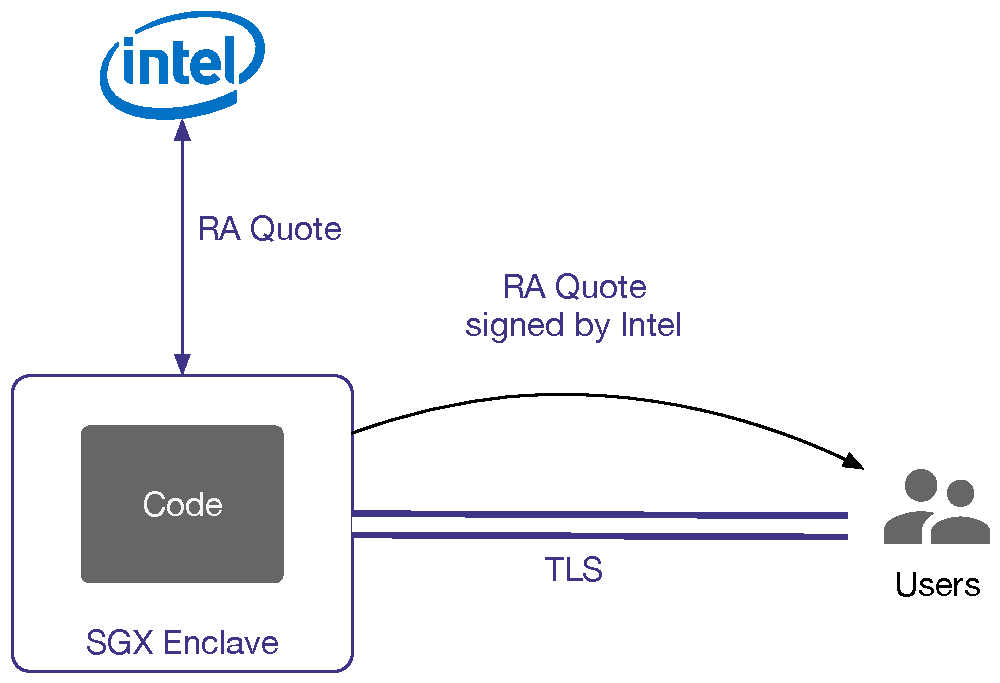
\includegraphics[width=.7\columnwidth]{img/pLIBRA-sgxra}
    \caption{Intel SGX remote attestation procedure.}
    \label{fig:sgx-ra}
\end{figure}

To ensure the execution is finished as expected inside an enclave, a proof can be generated according to a protocol called \textbf{Remote Attestation}. The hardware can generate an \textit{attestation quote} based on the details of hardware, firmware, the code being executed inside the enclave, and other user-defined data produced by the code. The quote is signed by the trusted hardware with credentials embedded during the production process.

Next, the generated attestation quote is sent to the Intel Remote Attestation Service. Intel will sign the quote iff the signing credentials are valid. As each credential is uniquely bound to an Intel CPU unit, fake attestation quotes will never pass the Remote Attestation Service check.

Finally, the attestation quote signed by Intel serves as the proof of successful execution. It proves that specific code has been run inside an SGX enclave and produces certain output, which implies the confidentiality and the correctness of the execution. The proof can be published and validated by anyone with generic hardware.

Intel SGX and the Remote Attestation protocol is the foundation of Confidential Contract. Except for Intel SGX, there are also alternative implementation choices like AMD SEV~\cite{xxx} and ARM TrustZone~\cite{xxx}.

\subsection{Event Sourcing and CQRS}

% Event Sourcing means we use the blockchain to record events (tx) to retain their order.
% CQRS means the commands (write ops) are put into the blockchain but the queries (read ops) can be made by runtime directly, improving the scalability of the contracts.

\hang{Should we create a subsection for this? I don't think we have a lot to tell here.}